\section{Các cải tiến đề xuất}
\label{sec:improvements}

Dựa trên reimplementation của thuật toán Rosiles và Smith \cite{rosiles2000}, chúng tôi đề xuất ba cải tiến nhằm nâng cao chất lượng denoising và giảm thiểu một số hạn chế của phương pháp gốc. Các cải tiến được thiết kế độc lập và có thể kết hợp với nhau.

% -----------------------------------------------------------------------
\subsection{Cải tiến 1: BayesShrink thay cho SURE/GCV}
\label{subsec:improve_bayes}

\subsubsection{Hạn chế của SURE và GCV}

SURE và GCV là các phương pháp ước lượng threshold hoàn toàn data-driven, không cần prior về phân phối tín hiệu. Tuy nhiên, trong bối cảnh DFB denoising, chúng có một số hạn chế:

\begin{itemize}
    \item \textbf{Độ phức tạp tính toán:} Cả SURE và GCV đều cần sắp xếp tất cả hệ số và tính tổng tích lũy, với độ phức tạp $O(n \log n)$, trong đó $n = M \times N$ là tổng số pixel (bằng kích thước ảnh với undecimated DFB). Với ảnh lớn, chi phí này trở nên đáng kể khi tính cho cả $N$ subband.

    \item \textbf{Nhạy cảm với outlier:} SURE giả định noise Gaussian thuần túy; nếu có outlier trong subband (do signal strength lớn), ước lượng SURE có thể bị bias về threshold nhỏ, dẫn đến under-thresholding.

    \item \textbf{Không khai thác thông tin per-subband:} SURE và GCV chỉ dùng phân phối hệ số để ước lượng threshold, không tận dụng sự khác biệt về signal strength giữa các subband --- một thông tin quan trọng khi các directional subband có mức độ tập trung năng lượng tín hiệu khác nhau.
\end{itemize}

\subsubsection{BayesShrink cho DFB}

BayesShrink \cite{chang2000}, ban đầu được thiết kế cho DWT, giả định signal trong mỗi subband có phân phối Laplacian (generalized Gaussian với tham số hình dạng $p = 1$), phù hợp với phân phối heavy-tailed điển hình của các hệ số ảnh thực. Dưới giả định này, threshold tối ưu theo tiêu chí Bayes risk (MMSE) là:

\begin{equation}
    t_k^* = \frac{\sigma_k^2}{\sigma_{x,k}}
    \label{eq:bayes_dfb}
\end{equation}

trong đó $\sigma_k$ là noise standard deviation của subband $k$ (theo \eqref{eq:sigma_k}), và $\sigma_{x,k}$ là signal standard deviation ước lượng từ subband:

\begin{equation}
    \sigma_{x,k} = \sqrt{\max\!\bigl(\sigma_{y,k}^2 - \sigma_k^2,\; 0\bigr)}
    \label{eq:sigma_x}
\end{equation}

với $\sigma_{y,k}^2 = \operatorname{var}(y_k^{\text{HP}})$ là phương sai quan sát được của subband. Khi $\sigma_{y,k}^2 \leq \sigma_k^2$ (subband là noise-dominated), $\sigma_{x,k} = 0$ và threshold được đặt bằng $\max|y_k^{\text{HP}}|$ để xóa toàn bộ subband.

Ưu điểm của BayesShrink so với SURE/GCV trong bối cảnh này:
\begin{itemize}
    \item \textbf{Adaptive per-subband:} Threshold tự động điều chỉnh theo signal strength của từng directional subband --- subband giàu tín hiệu (cạnh theo hướng tương ứng) có $\sigma_{x,k}$ lớn nên threshold nhỏ (bảo tồn tín hiệu), trong khi subband nghèo tín hiệu có threshold lớn (denoising aggressive).
    \item \textbf{Độ phức tạp $O(n)$:} Chỉ cần tính variance của subband, không cần sort.
    \item \textbf{Robust hơn với non-sparse subbands:} Cơ chế variance estimation ít nhạy cảm hơn với outlier so với argmin search của SURE.
\end{itemize}

% -----------------------------------------------------------------------
\subsection{Cải tiến 2: Tăng số band lên 16 (angular resolution)}
\label{subsec:improve_16band}

\subsubsection{Động lực}

Trong paper gốc \cite{rosiles2000}, DFB 8 band được sử dụng, tức là mỗi directional subband bao gồm một dải góc rộng $\Delta\theta = 180°/8 = 22.5°$. Với các ảnh có texture hoặc cạnh theo nhiều hướng gần nhau (ví dụ: ảnh SAR với sóng biển, ảnh y tế với thớ cơ), độ phân giải góc $22.5°$ có thể không đủ mịn để phân tách signal và noise hiệu quả.

\subsubsection{DFB 16 band}

Chúng tôi đề xuất tăng số band lên $N = 16$, giảm bandwidth mỗi band xuống $\Delta\theta = 180°/16 = 11.25°$. Các filter vẫn được thiết kế theo công thức raised-cosine với overlap $1.2\Delta$ và chuẩn hóa partition-of-unity như mô tả trong Mục~\ref{subsec:undecimated}. Số band $N = 16$ vẫn là lũy thừa của 2, tương thích với cấu trúc binary tree của DFB gốc (tương đương $l = 4$ tầng).

Với $N = 16$ band, mỗi directional subband tập trung năng lượng của một dải hướng hẹp hơn, cho phép:
\begin{itemize}
    \item Phân tách tốt hơn các texture theo các hướng gần nhau.
    \item Threshold per-subband có tính selective hơn: chỉ các subband đúng hướng của cạnh mới có signal strength cao.
    \item Potentially higher PSNR trên các ảnh giàu directional content.
\end{itemize}

Chi phí là tăng gấp đôi số lượng DFT/IDFT cần tính (từ $8$ lên $16$ lần), nhưng với undecimated DFB, chi phí này vẫn tuyến tính theo $N$ và chấp nhận được.

\begin{figure}[H]
    \centering
    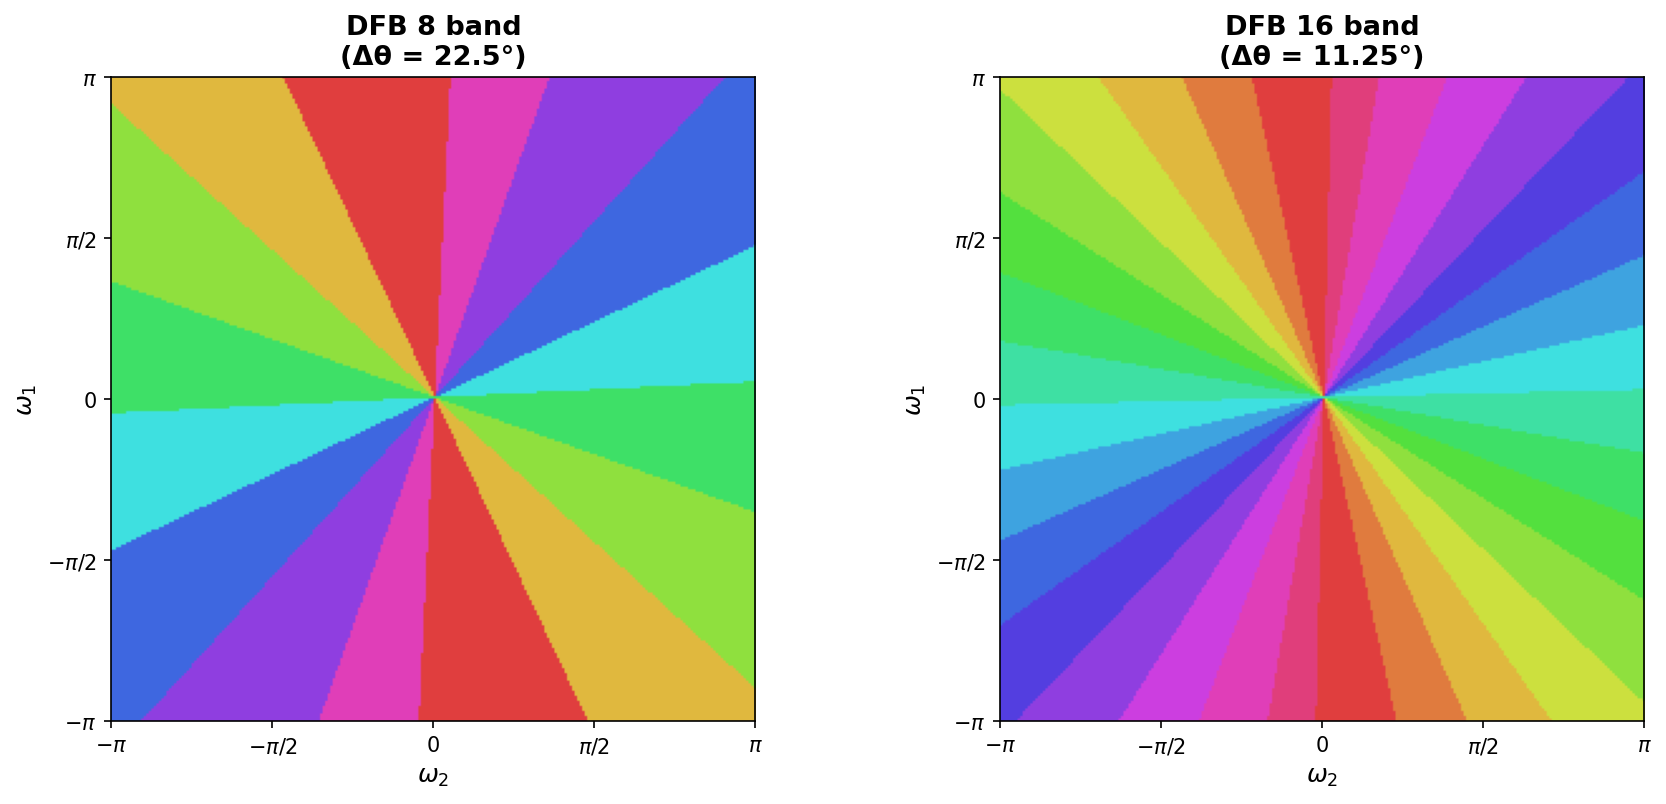
\includegraphics[width=0.85\textwidth]{figures/dfb_8vs16_comparison.png}
    \caption{So sánh phân chia mặt phẳng tần số của DFB 8 band (trái) và DFB 16 band (phải).
             Mỗi màu đại diện cho một directional subband. DFB 16 band có độ phân giải góc mịn hơn ($11.25°$ so với $22.5°$).}
    \label{fig:dfb_16band}
\end{figure}

% -----------------------------------------------------------------------
\subsection{Cải tiến 3: Multi-scale undecimated DFB}
\label{subsec:improve_multiscale}

\subsubsection{Động lực}

Một hạn chế quan trọng của DFB đơn scale là không có phân tích đa tần số: mọi cấu trúc hướng (coarse hay fine) đều được phân tích ở cùng một độ phân giải. Trong khi đó, cạnh và texture thực tế xuất hiện ở nhiều scale khác nhau --- cạnh sắc ở scale mịn, cấu trúc lớn ở scale thô. Wavelet transform giải quyết điều này bằng multi-resolution analysis, nhưng DWT chỉ có ba hướng cố định tại mỗi scale.

\subsubsection{Kiến trúc multi-scale}

Chúng tôi đề xuất kết hợp Gaussian pyramid với DFB tại mỗi scale, tạo ra một multi-scale undecimated DFB. Kiến trúc này có quan hệ mật thiết với Contourlet transform \cite{do2005}.

Cụ thể, ảnh nhiễu $y$ được phân tích thành $L$ band-pass layer và một coarsest approximation:

\begin{equation}
    y = b_0 + b_1 + b_2 + \cdots + b_{L-1} + a_L
    \label{eq:pyramid}
\end{equation}

trong đó:
\begin{align}
    a_0 &= y \\
    a_l &= G_{2^l} * y, \quad l = 1, \ldots, L \\
    b_l &= a_{l-1} - a_l = (G_{2^{l-1}} - G_{2^l}) * y, \quad l = 1, \ldots, L
\end{align}

Mỗi $b_l$ là một Gaussian bandpass layer, tập trung năng lượng ở một dải tần số nhất định (scale $l$). Do không có decimation, mỗi $b_l$ có cùng kích thước với ảnh gốc và phân tích \eqref{eq:pyramid} là lossless: $\sum_l b_l + a_L = y$.

Với mỗi bandpass layer $b_l$, DFB được áp dụng để phân tách theo hướng:

\begin{equation}
    b_l = \sum_{k=0}^{N-1} b_{l,k}
\end{equation}

Mỗi $b_{l,k}$ là một directional-scale subband, tập trung năng lượng ở scale $l$ và hướng $k$. Thresholding được thực hiện độc lập cho từng $b_{l,k}$:

\begin{equation}
    \hat{b}_{l,k} = \eta_{t_{l,k}}(b_{l,k})
\end{equation}

Ảnh tái tạo cuối cùng là:

\begin{equation}
    \hat{x} = a_L + \sum_{l=1}^{L} \sum_{k=0}^{N-1} \hat{b}_{l,k}
    \label{eq:multiscale_recon}
\end{equation}

\begin{figure}[H]
    \centering
    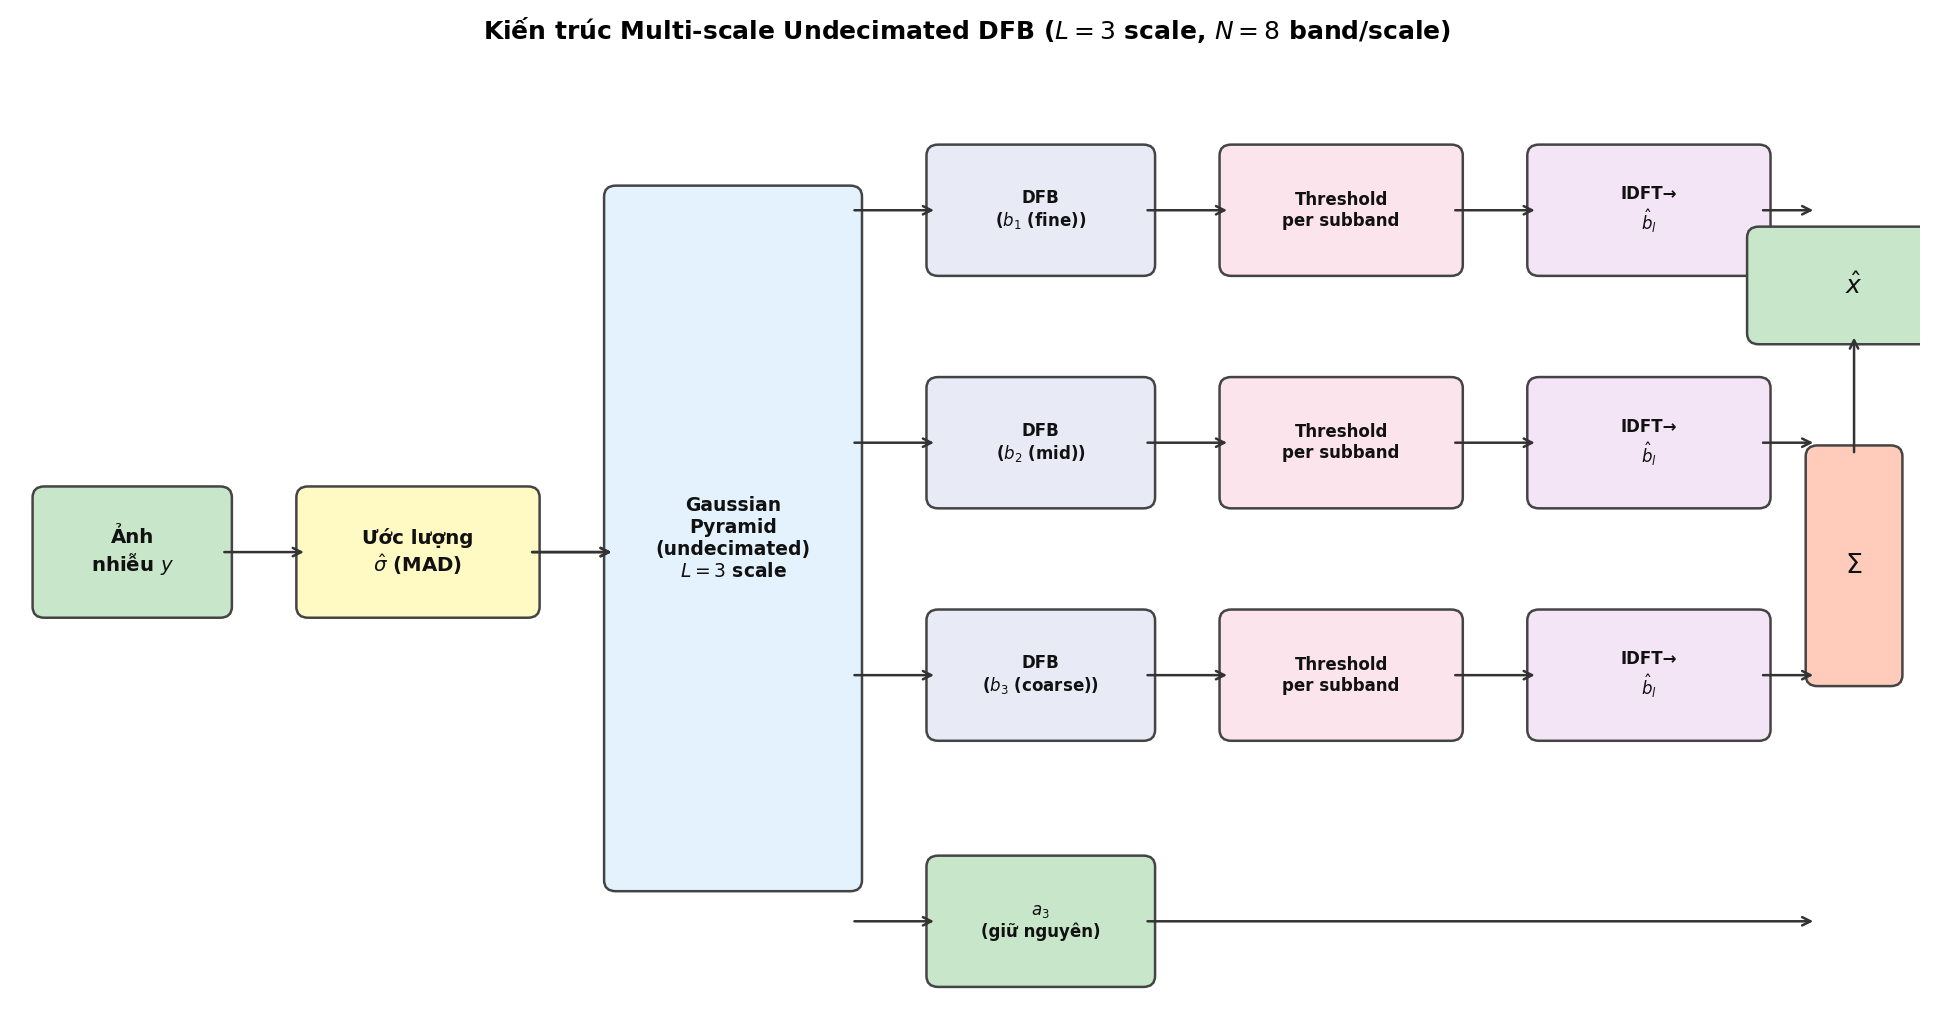
\includegraphics[width=0.9\textwidth]{figures/multiscale_diagram.png}
    \caption{Kiến trúc multi-scale undecimated DFB với $L = 3$ scale và $N = 8$ directional band.
             Mỗi bandpass layer $b_l$ được phân tách thành $N$ directional subband, tạo ra $L \times N$ subband tổng cộng.
             Coarsest approximation $a_L$ được giữ nguyên không qua thresholding.}
    \label{fig:multiscale}
\end{figure}

\subsubsection{Ước lượng sigma per-scale}

Noise sigma tại mỗi scale được ước lượng riêng từ bandpass layer tương ứng. Do $b_l$ là kết quả của bandpass Gaussian filter với bandwidth tỷ lệ với $2^{-l}$ (scale thô hơn có bandwidth hẹp hơn), noise power trong $b_l$ phụ thuộc vào bandwidth:

\begin{equation}
    \sigma_{b_l}^2 \approx \sigma^2 \cdot \int |G_{2^{l-1}}(\omega) - G_{2^l}(\omega)|^2\, d\omega
\end{equation}

Trong thực tế, chúng tôi ước lượng $\sigma_{b_l}$ trực tiếp từ layer $b_l$ bằng MAD estimator, cho phép tự động thích ứng với noise distribution tại mỗi scale. Per-subband sigma sau đó là $\sigma_{l,k} = \sigma_{b_l}/\sqrt{N}$.

\subsubsection{So sánh với Contourlet transform}

Multi-scale undecimated DFB của chúng tôi có quan hệ mật thiết với Contourlet transform \cite{do2005}. Contourlet cũng kết hợp Laplacian pyramid (LP) với DFB tại mỗi scale, nhưng sử dụng decimated LP pyramid (downsampling 2:1 sau mỗi tầng) thay vì undecimated Gaussian pyramid. Sự khác biệt chính:

\begin{itemize}
    \item \textbf{Redundancy:} Undecimated DFB của chúng tôi là overcomplete (mỗi scale có $N$ subband với kích thước ảnh gốc), trong khi Contourlet là critically-sampled (tổng số hệ số bằng số pixel).
    \item \textbf{Shift-invariance:} Undecimated DFB shift-invariant hoàn toàn; Contourlet không shift-invariant do decimation.
    \item \textbf{Reconstruction:} Cả hai đều hỗ trợ perfect reconstruction, nhưng Contourlet đòi hỏi thiết kế filter cẩn thận hơn.
\end{itemize}

Shift-invariance là lợi thế quan trọng trong denoising: các phương pháp không shift-invariant (như DWT và Contourlet gốc) thường tạo ra pseudo-Gibbs artifact ở vùng lân cận cạnh.

% -----------------------------------------------------------------------
\subsection{Tóm tắt các cải tiến}

Bảng~\ref{tab:improvements} tóm tắt ba cải tiến đề xuất so với phương pháp gốc.

\begin{table}[H]
    \centering
    \caption{So sánh các cải tiến với phương pháp gốc Rosiles \& Smith \cite{rosiles2000}.}
    \label{tab:improvements}
    \begin{tabular}{@{}lllll@{}}
        \toprule
        \textbf{Phương pháp} & \textbf{Threshold} & \textbf{Số band} & \textbf{Multi-scale} & \textbf{Shift-inv.} \\
        \midrule
        Gốc (Rosiles \& Smith) & SURE / GCV & 8 & Không & Không \\
        Cải tiến 1 & BayesShrink & 8 & Không & Có \\
        Cải tiến 2 & SURE / GCV & 16 & Không & Có \\
        Cải tiến 3 & BayesShrink & 8 & Có ($L=3$) & Có \\
        \bottomrule
    \end{tabular}
\end{table}
